% Chapter Template

\chapter{Experiment Methodology} % Main chapter title

\label{Chapter5} % Change X to a consecutive number; for referencing this chapter elsewhere, use \ref{ChapterX}

\lhead{Chapter 5. \emph{Experiment Methodology}} % Change X to a consecutive number; this is for the header on each page - perhaps a shortened title

%----------------------------------------------------------------------------------------
%	SECTION 1
%----------------------------------------------------------------------------------------

\section{Models}

The experiment setup and results for all the models - Black-Scholes, Vanilla Neural Network and Combined Neural Network, have been dicussed in this section.

\subsection{Black-Scholes}

To compare the results of the proposed neural network model, Black-Scholes is used as a baseline model.

\begin{figure}[htbp]
  \centering
    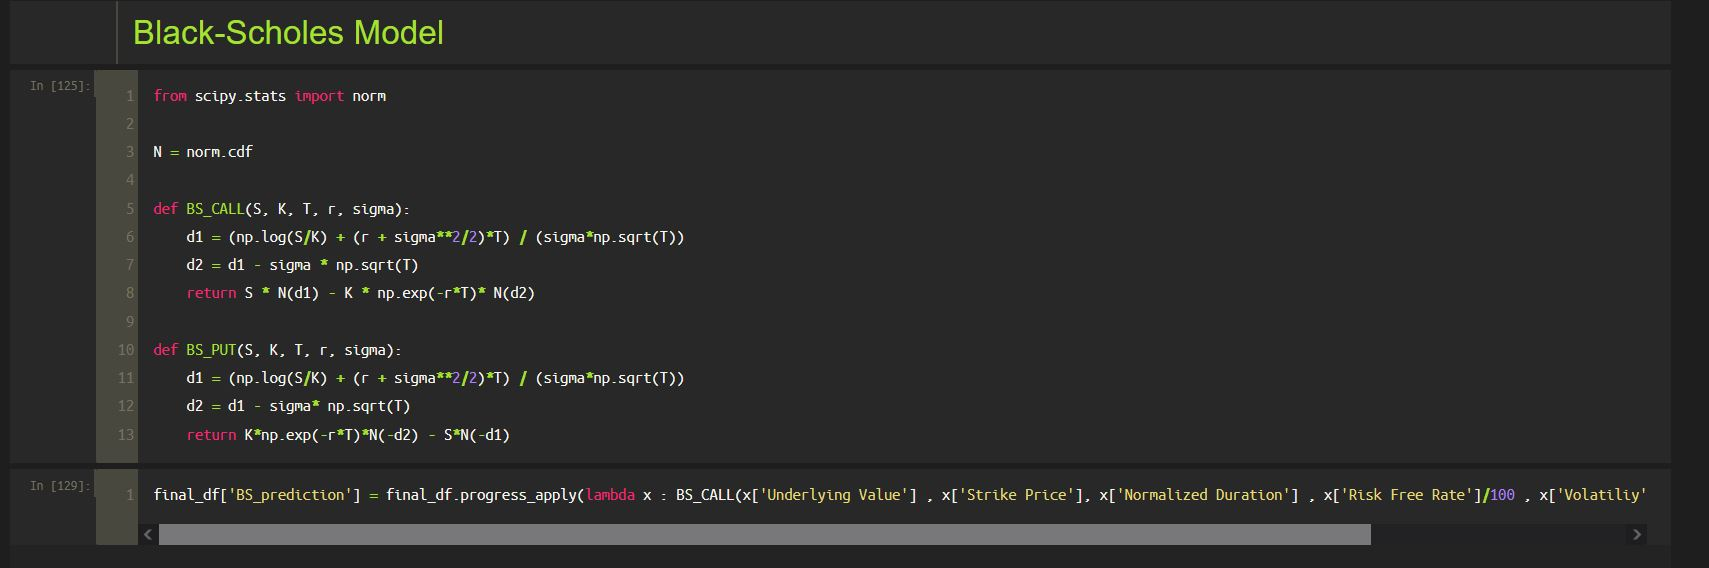
\includegraphics[scale=0.45]{Figures/bs_model.JPG}
    \rule{35em}{0.5pt}
  \caption[Black-Scholes Code]{Black-Scholes Code}
  \label{fig:bs_code}
\end{figure}

\subsection{Vanilla Neural Network}

The first architecture is a feed forward neural network having 4 hidden layers where the first hidden layer contains 40 neurons, the next three contain 100 neurons each and the output layer contains a single neuron which outputs the option premium.

\begin{figure}[htbp]
  \centering
    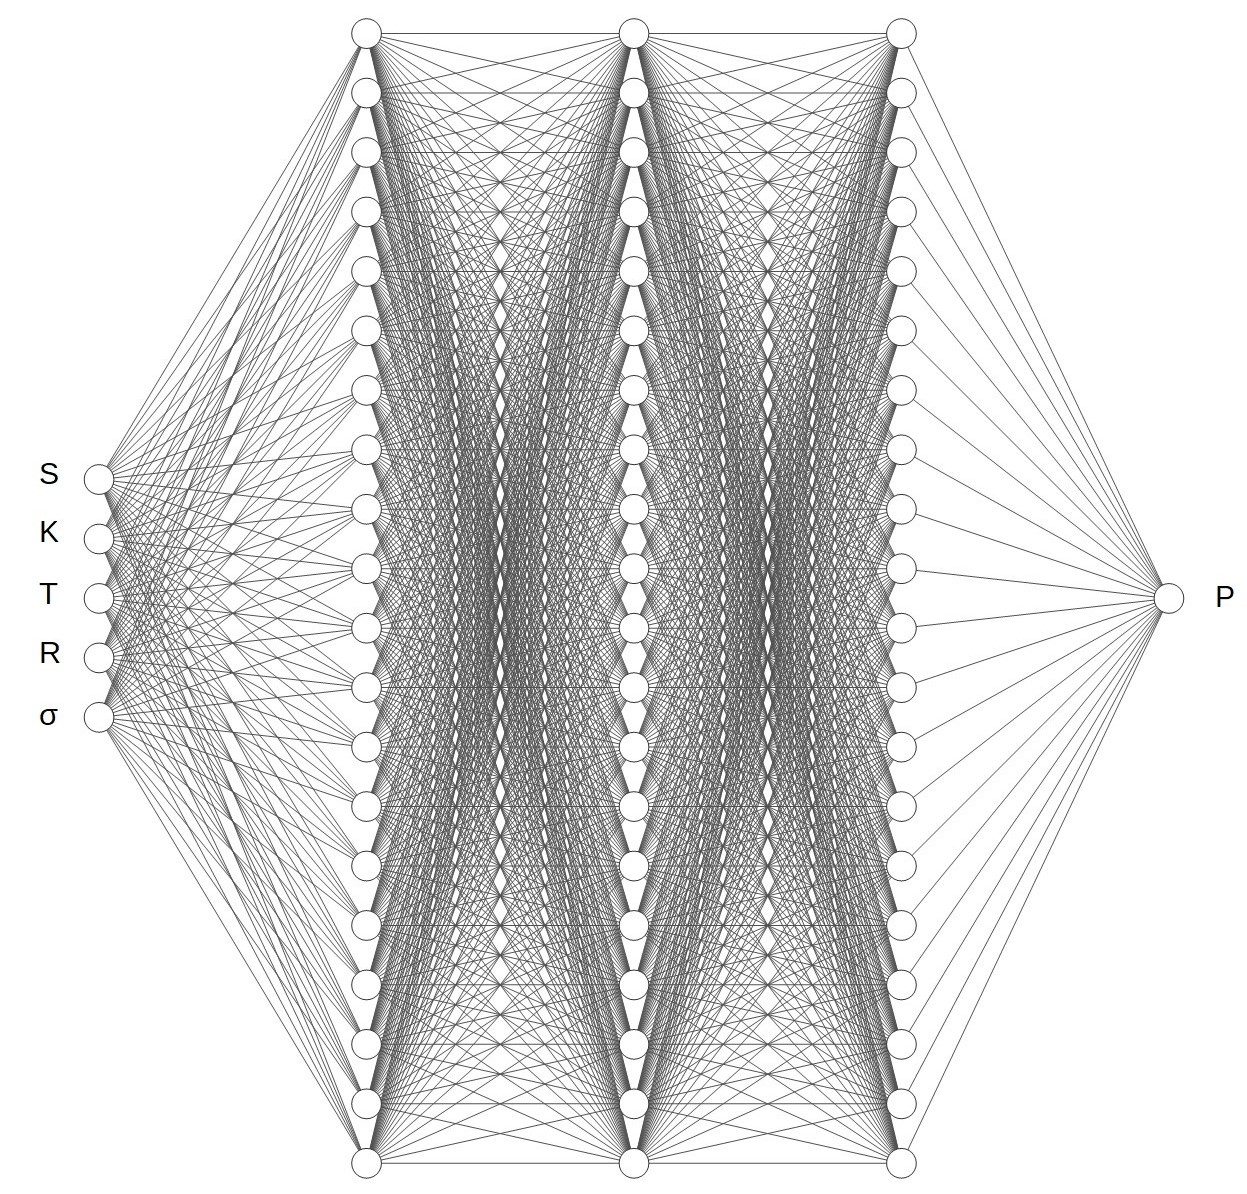
\includegraphics[scale=0.45]{Figures/model_1_vnn.jpg}
    \rule{35em}{0.5pt}
  \caption[Vanilla Neural Network - Architecture]{Vanilla Neural Network - Architecture}
  \label{fig:model_1_vnn}
\end{figure}

The inputs for this model are:
\begin{itemize}[noitemsep,topsep=0pt]
    \item Current Asset Price (S)
    \item Strike Price (K)
    \item Duration till expiry (T)
    \item Risk Free Rate (R)
    \item Historic Volatility ($\sigma$)
\end{itemize}

This model is trained on put and call option data separately. 


\subsection{Combined Neural Network}

This model is very similar to the Vanilla Neural Network, except for a small difference. Apart from the inputs available in the previous model, an additional input which signifies the option category is also present in this architecture. Call options are given category as '1' and put options as '0'. Incorporating this small change allows us to train the model on all the option data, without having to train put and call models separately.

\begin{figure}[htbp]
  \centering
    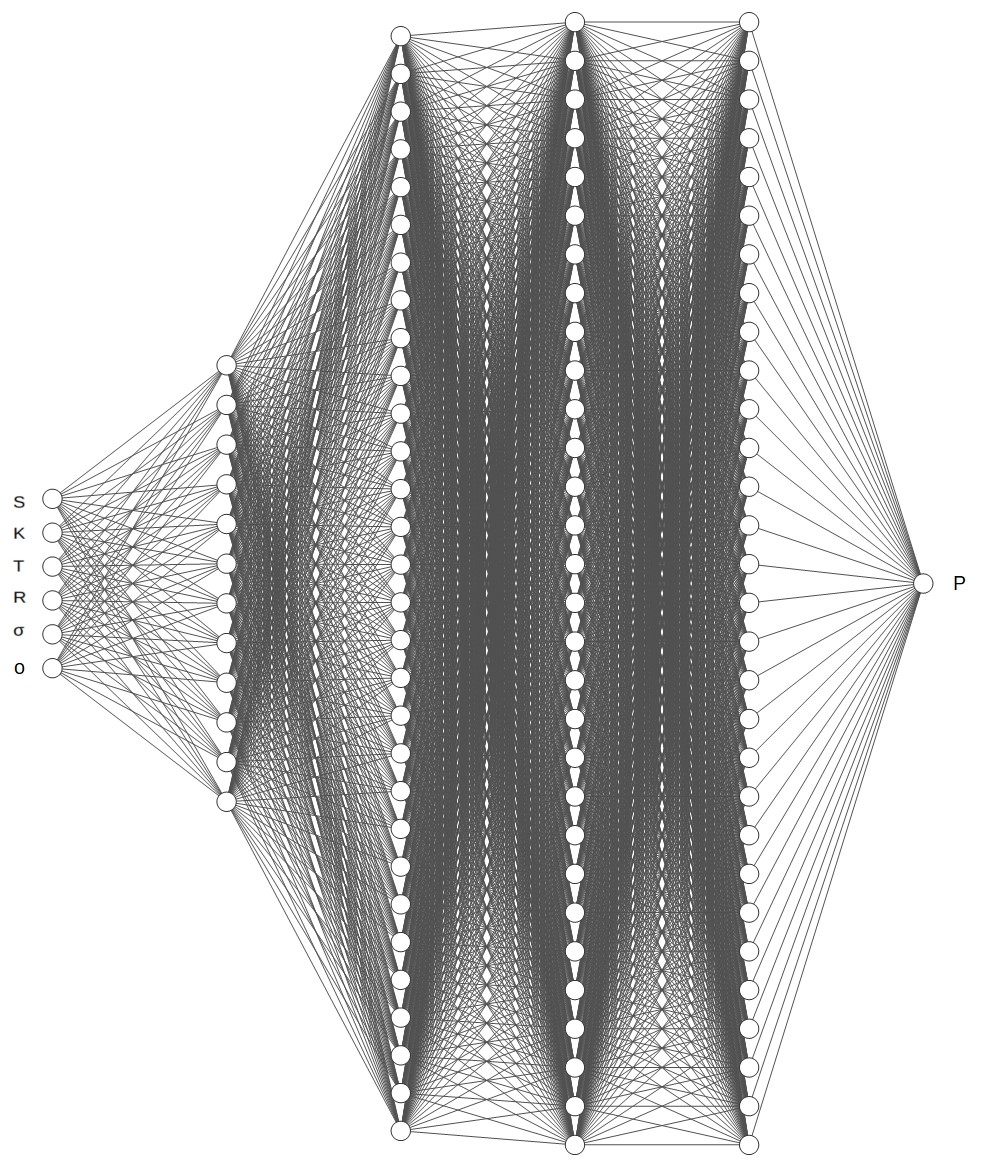
\includegraphics[scale=0.45]{Figures/model_2_combined.jpg}
    \rule{35em}{0.5pt}
  \caption[Combined Neural Network - Architecture]{Combined Neural Network - Architecture}
  \label{fig:model_2_combined}
\end{figure}
